\begin{savequote}[75mm]

... As for me, nothing in the universe can be the same if somewhere, no one knows where, a sheep we never saw has or has not eaten a rose....
Look up at the sky. Ask yourself, ``Has the sheep eaten the flower or not?" And you'll see how everything changes....
And no grown-up will ever understand how such a thing could be so important!
\qauthor{Antoine de Saint-Exup{\^e}ry (The Little Prince)}
\end{savequote}


\chapter{Introduction}
\label{introduction}

\section{A Brief History of Galaxy Evolution}

\subsection{The Discovery of Galaxies}
One of the momentous shifts in scientific thinking was the realization that our Sun might be one of many stars in the Universe. From this sprung the idea that perhaps the gravitationally bound system of stars, stellar remnants, gas and dust that the Sun is a part of is one of many such structures known as galaxies. The bright band of stars and dust that we observe in the night sky, which we now know as our own galaxy, the Milky Way, has been a puzzling topic since ancient times. The Greek philosopher Democritus is known to have speculated that this might be a band of distant stars but the thought was left by the wayside with the advent of Aristotelian physics. The astronomers of medieval Islam, such as Alhazen, al-Biruni and Ibn-Bajjah, centuries later, also hypothesized that the Milky Way was made of many stars such as our own Sun. However, observational proof for this came only in the 17th century when the Italian astronomer, Galileo Galelei pointed his telescope at this band and confirmed that the Milky Way was indeed made up of a huge number of faint stars.\\

Since the debate on a geocentric versus heliocentric Universe was still ongoing, Galileo's observations weren't given credence until more than century later, during which time, the development of Keplerian orbital mechanics and Newtonian Theory of Gravitation had resulted in a successful explanation of the Solar System and its dynamics. The idea that the galaxy might be a rotating configuration of a huge number of stars held together by gravitational forces that contained smaller gravitationally bound configurations such as our Solar System was first theorized by the English astronomer, Thomas Wright, in 1750. On the heels of his observation that the faint (then so-called) ``nebulae" observed might be distant galaxies that came out of ``external creations", philosopher Immannuel Kant hypothesized the existence of many such ``island Universes" and speculated that these could potentially form and evolve independently from our own, thus laying the underpinnings of the study of galaxy formation and evolution.\\

\subsection{Early Studies of Galaxies}

William Herschel, in the 1780s, surveyed the stars in the Milky Way in multiple directions and discovered that the density of stars was greater on one side than the other. One of the earliest catalogues of galaxy-like objects was developed by Charles Messier, also towards the end of the 18th century, following which William Herschel assembled a catalog of 5000 nebulae. In the 19th century, with advances in optics and instrumentation, the first telescope to distinguish between elliptical and spiral galaxies was built by Lord Rosse. Additionally, this telescope could resolve point sources within the nebulae, thus confirming that galaxies were indeed ``island universes" as Wright and Kant had surmised.\\

In early 20th century, astronomers were beginning to get interested in the chemical composition of these nebulae and started recording their spectra. With the advent of Einstein's Special Theory of Relativity, one could calculate the radial velocity of a ``nebula" based on how its spectrum is Doppler-shifted. And so it happened that the American astronomer, Vesto Slipher, became the first person to measure galactic redshifts in 1912. While studying the chemical composition of bright spiral nebulae, he noticed that they were all highly Doppler-shifted, with estimated radial velocities that were much higher than the velocities of stars in the Milky Way. He also noticed that there were more ``red-shifted" (i.e. moving away from us) nebulae than ``blue-shifted" ones, an observation that would later propel Edwin Hubble to propose that the Universe was expanding.\\

In the 1920s, a series of observations made by Edwin Hubble, Ernst Opik, etc., confirmed that Andromeda was not a part of the Milky Way and was a galaxy is its own right, thus effectively settling the ``Great Debate" of the times and confirming that our galaxy was just one of many galaxies in the Universe. Georges Lema{\'i}tre, a Belgian physicist, predicted, on theoretical grounds rooted in Einstein's General Theory of Relativity, that the redshifts of galaxies should increase with distance. In 1929, Edwin Hubble looked at the distances and velocities of 46 galaxies and observed the same \citep{1929PNAS...15..168H}: that their radial velocities increased with distance from us, thus theorizing what we know today as Hubble's Law (or alternately, the Hubble-Lema{\'i}tre Law). Edwin Hubble further analyzed the morphologies of these galaxies and came up with the Hubble Sequence, a classification of galaxy morphology (Fig. \ref{fig:hubble_classification}). The Swiss astrophysicist, Fritz Zwicky, in 1933, while studying galaxy clusters, noticed that the orbits of the galaxies were not accounted for by the mass of its luminous components, leading him to believe that there must be some ``missing" mass \citep{1937ApJ....86..217Z} that does not interact electromagnetically, thus remaining unseen and termed it \emph{dunkle Materie}, i.e.,``dark matter".\\

Thus with the emergence of new theories of spacetime, an expanding Universe that (as it was termed later) began with a ``big bang", the existence of matter that doesn't interact electromagnetically, the study of galaxies in the 1930s set in motion a paradigm shift for astronomy and cosmology. The new questions were: How were the earliest galaxies formed? What would explain the diversity in morphologies seen in galaxies today? Is the Universe set to expand indefinitely? What drives the expansion of the Universe? What is dark matter? If the Universe's origins were homogeneous, how do we explain the heterogenous nature of the populations of galaxies seen?\\

\subsection{Galaxy Evolution and Cosmology}

The explorations in the latter half of the 20th century confirmed a few of the hypotheses discussed above, along with answering a few of those questions. In the 1960s and 1970s, Vera Rubin, Kent Ford, and Ken Freeman analyzed rotation curves of spiral galaxies and provided strong evidence for the existence of dark matter \citep{freeman_disks_1970-1}. Rubin inferred that most galaxies contain around six times as much dark matter as visible mass \citep{rubin_rotational_1980}, thus placing new constraints on galaxy formation and evolution in the Universe.\\

The two predominant theories of the origin of the Universe were: the ``Big Bang Theory", originally proposed by Georges Lema{\'i}tre, and the ``Steady State Theory" (essentially an unchanging Universe whose density remains the same in spite of expansion due to continuous creation of matter) proposed by Fred Hoyle. However, with theories of Big Bang Nucleosynthesis (the $\alpha\beta\gamma$ paper; \citealt{alpher_origin_1948}) that successfully explained how the elements of the of the Universe came to be formed after the Big Bang and radio source counts which were also correctly accounted for by the Big Bang Theory swung cosmologists to favor this over the Steady State Theory. The final nail in the coffin was the successful detection of the Cosmic Microwave Background (CMB), predicted by the Big Bang Theory \citep{1965ApJ...142..419P}. According to the Big Bang Theory, the early Universe cools from a very hot state and remains an ionized plasma for the first few hundred thousand years (until redshift $z\sim 1100$). The emission from this era should be a Planck spectrum of the plasma at about the time that hydrogen recombines, redshifted due to the universe's expansion since then. This model predicts a spectrum peaking at near microwave wavelengths today, and the CMB is indeed detectable as a very low energy radiation with a blackbody temperature of \~ 3K.\\

The discovery of dark matter coupled with the confirmation of the Big Bang Theory necessitated a theory of dark matter that would successfully explain the observable Universe. In the 1980s, competing theories of hot and cold dark matter \citep{1985ApJ...292..371D} were proposed. Eventually the cold dark matter theories won out as their prediction of the anisotropies in the CMB \citep{peebles_large-scale_1982} were successfully verified by the Cosmic Background Explorer (COBE) probe \citep{smoot92a} in combination with other data sets.\\

Before the turn of the century, the remarkable discovery of the accelerating universe \citep{Riess:1998cb} resulted in the resurrection of Einstein's cosmological constant and effectively confirmed $\Lambda$CDM as the clear winner among the cold dark matter models. The Big Bang Theory, together with the $\Lambda$CDM model, forms much of the basis of modern cosmology and the foundations for theories of galaxy formation and evolution.\\

\section{Galaxy Formation and Evolution}

\subsection{Structure Formation in the Universe}
The current model of cosmology suggests that there was a single event, the so-called ``Big Bang" which resulted in the appearance of expanding space-time containing radiation, followed by an exponential expansion of space known as cosmic inflation \citep{PhysRevD.23.347} which established the initial properties of the Universe as being homogeneous, isotropic and flat. Tiny perturbations in this early Universe are responsible for structure formation. Cosmic inflation also explains the fact that these tiny quantum fluctuations grow into slight ripples of over-density and under-density thus seeding the early stages of structure formation in the Universe.\\

From a predominantly radiation-dominated Universe, with expansion, the density of radiation drops steeply leading to a the matter-radiation equality at ~ 50,000 years after the Big Bang. Since dark matter only interacts gravitationally, the dark matter ripples from the fluctuations form compact structures more freely as they are not opposed by other forces such as radiation pressure.\\

About 380,000 years after the Big Bang, the expansion of the Universe resulted in a lowering of density as well as a cooling down of its temperature to a point where protons and electrons in this plasma soup start combining to form the neutral hydrogen. Electrons decouple from the photons (these decoupled photons are what we detect as the CMB today) and the baryonic matter is now free to collapse under gravity creating local over-densities.\\

As fluctuations continue to grow, ever larger scales enter the non-linear regime of structure formation where dense concentrations of matter (dark and baryonic alike) get progressively denser. 
Dark matter begins to collapse into structures known as halos, and baryons fall with the dark matter into these halos. These structures arrange themselves into gravitationally stable configurations, a process known as virialization.
The result of this process gives rise to a Universe that resembles a web (the cosmic web) with sheets and filaments of dark matter, creating a skeletal backbone in which star formation and galaxy formation eventually occur.

Within the dark matter halos baryonic matter can, when it becomes dense enough, additionally lose energy by radiation and can sink further into regions of high over-density. 
The stars and galaxies have their origins in these structures and are the resulting of the cooling of baryons deep in the potential wells of dark matter halos.

While a short summary of how galaxies form would be that the collapse of baryonic matter within dark matter halos results in disk-like structures that then collapse on small scales to form stars, the mechanisms by which this happens is still a topic of debate among astrophysicists. While a top-down scenario, wherein disk galaxies were formed from the collapse of a single large cloud of gas \citep{1962ApJ...136..748E}, captures some stages of galaxy formation well, in fact both theory and observations suggest that galaxies grow hierarchically --- small galaxies form and merge into larger ones --- which complexifies the picture. Meanwhile, the overall efficiency with which baryons form stars depends strongly on the halo mass (e.g. \citealt{behroozi_comprehensive_2010}), peaking at masses similar to that of the Milky Way. As \citet{somerville15a} describe, this dependence probably arises from processes that suppress star formation at lower masses (perhaps due to supernova feedback) and at higher masses (perhaps due to feedback from accreting supermassive black holes).

% Prior to the establishment of $\Lambda$CDM as the dominant cosmological model, the popular theory of galaxy formation was the top-down scenario \citep{1978ApJ...225..357S} which proposed that disk galaxies were formed from the collapse of a single large cloud of gas \citep{1962ApJ...136..748E} into disks that pushed the dark matter out into halos. The cooling of this rotating disk results in gravitational instabilities that causes smaller clumps of clouds to collapse to form stars. However, the natural prediction of $\Lambda$CDM is a bottom-up scenario wherein the dark matter halos form and 
% (\citet{0004-637X-490-2-493, 2015PNAS..11212249W}) before the formation of the galactic disks.\\

Since we are limited in our observations by the fact that we cannot observe galaxies in a time-resolved fashion (the time scales are too long), theories regarding galaxy formation rely computational simulations that evolve the initial conditions to the present day. We can compare the galaxies at each epoch to the populations observed at different redshift, assuming large scale homogeneity. As \citet{somerville15a} describe, these simulations incorporate the physics of $\Lambda$CDM, magnetohydrodynamics, and gravitation. Additionally, these models need to account for a variety of processes on subresolution scales that involve star formation, stellar and AGN feedback, and gas cooling to be able to correctly predict the observed Universe.\\

\begin{figure}
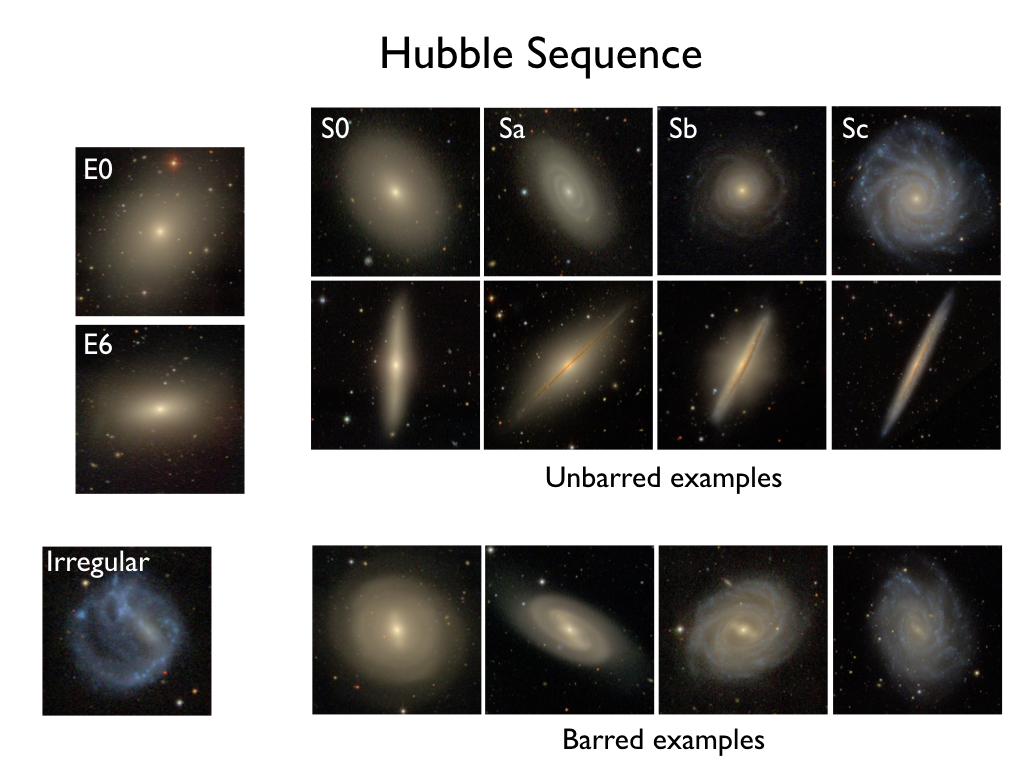
\includegraphics[width=\textwidth]{figures/hubble.jpeg}
\caption[ The Hubble Sequence: A classification scheme for galaxy morphologies (Photo credit: ?)]
{The Hubble Sequence: A classification scheme for galaxy morphologies (Photo credit: ?)
\label{fig:hubble_classification}}
\end{figure}

Thus, there are still many questions to be answered including and not limited to: how and where the baryons collapse, how galactic disks stabilize, the drivers and mechanisms of galactic feedback and what ultimately causes the relative frequency of different galaxy types in the observable Universe. There are thus many holes in this narrative of galaxy formation and evolution and astronomers are working to bridge this gap in two main ways: from the observational side, this involves accurate measurements of galaxy properties across cosmic time and from the (theoretical) side of computational astrophysics, this involves fine-tuning the sub-grid models of galaxy formation and evolution simulations so as to be able to reproduce the estimated from the properties. These both take from and in turn inform the parameters in the $\Lambda$CDM model of the Universe that cosmologists are engaged in refining.\\

\subsection{Galaxy Properties in the Observable Universe}

The commonly used classification scheme for galaxies based on their most obvious attribute, the morphologies of their luminous components, was invented by Edwin Hubble in 1926. The classification scheme is based on the relative sizes and of the bulges and disks in galaxies and broadly encompasses four types of morphologies: elliptical, lenticular, spiral and irregular (Fig. \ref{fig:hubble_classification}). Galaxy morphologies are strongly correlated with their other physical properties such as luminosity, age, chemical composition, star formation histories and kinematics (\citealt{roberts94a}). The bulges usually contain older, redder stars and the disks are characterized by mixed stellar populations along with gas and dust. The disks may also contain spiral arms which usually contain pockets of star formation activity. Elliptical galaxies have almost no disk. Lenticulars are smooth like ellipticals but contain a puffy, thick disk that when observed obliquely has a distinct oval-like appearance (lentil-shaped!). Spirals can have a bulge but are characterized by their thin disk, often with spiral arms. Irregulars are akin to spirals but as their name suggests, appear less organized in their light distribution. Early ideas about galaxy evolution suggested that galaxies formed as ellipticals or lenticulars (referred to as `early-type' galaxies) and later evolved into spirals or irregulars (referred to as `late-type' galaxies) and while there are strong correlations between galactic structure and their star formation rates, it is now known that this is in general untrue.\\

The total amount of light we observe emanating from a galaxy is the
second obvious trait that lends itself to comparison. This can be
quantified as ``luminosity,'' the amount of energy emitted by a star
per unit time, often measured in units of the solar luminosity
$L_{\odot}$, and usually measured in a particular wavelength
bandpass. Optical or near-infrared luminosity can serve as a
reasonable (but not exact) proxy for stellar mass; ultraviolet
luminosity can serve as a reasonable (but not exact) proxy for
current star formation activity. Observations reveal that fainter
galaxies are more frequent per unit volume than galaxies as bright
as our own. Very bright big ellipticals are much rarer than both.
The distribution of galaxy luminosites, per volume and per unit
luminosity, is known as the ``luminosity function''
(\citet{1988MNRAS.232..431E, blanton05a}), which provides key
constraints on galaxy formation and evolution.

The total luminosity of a galaxy in the ultraviolet through near
infrared is generally dominated by stars, and the stellar population
is changing with time as stars evolve off the main sequence and reach
their fates, for example as black holes, neutron stars, or white
dwarfs.  A more stable and sometimes more interesting quantity is the
total mass in stars, the stellar mass. Because the luminosities of
stars varies as $L\propto M^{-\alpha}$, where $\alpha \sim 3$--$5$,
and the more massive stars die rapidly, the total ratio of luminosity
to stellar mass varies over time. Furthermore, because the massive
stars are very hot, the overall color of the stellar population starts
out blue and becomes increasing red. This pattern leads to a
relationship between the galaxy spectrum and the stellar mass to light
ratio, that can be exploited to estimate the stellar mass of a galaxy.

The most basic measure of the spectral energy distribution of galaxies
are its colors.  Colors in astronomy are defined on the basis of the
ratios of observed fluxes in various bandpasses. For instance, $g-r$
is $2.5\log_{10}$ of the ratio of the $r$-band to $g$-band flux, where
$g$ and $r$ are optical bandpasses used in the Sloan Digital Sky
Survey (SDSS); larger $g-r$ indicates a redder galaxy.  Galaxy
populations have a bimodal distribution and can be divided into the
so-called ``red sequence" and ``blue cloud"
(\citet{2001AJ....122.1861S, 2003ApJ...594..186B}). The blue cloud is
dominated by star-forming blue spirals with young stellar populations;
the red sequence has a mixture of varied populations, including some
older or dust-reddened spirals, lenticular galaxies, and ellipticals.
The intermediate colored population, the so-called ``green valley",
must contain (but does not only contain) the population of galaxies
that are in the process of ending their star formation and
transitioning from blue to red. However, a complication to this simple
interpretation of the observations is the presence of dust, which has
the tendency to make galaxies appear redder. We investigate the star
formation of galaxies in the context of optical colors and dust,
further in Chapter \ref{ch:sfrk}.\\

The last significant observable property we introduce here is the
galaxy environment, which is a measure for each galaxy of how many
other galaxies are nearby it relative to the mean galaxy density.
Galaxies exhibit substantial clustering relative to a Poisson
distribution, leading to a large dynamic range in local density For
example, a galaxy like the Milky Way most commonly has not similarly
massive neighbors within 1 Mpc, but massive clusters of galaxies have
100s of Milky Way-sized galaxies within a Mpc. This clustering of
galaxies reveals information about cosmological parameters, like the
initial amplitude of fluctuations and the mean dark matter density.

The environment of galaxies also appears to be correlated with their
formation history, as manifested by their morphology
\citep{dressler_galaxy_1980}, luminosity \citep{2002MNRAS.332..827N},
star formation rates \citep{2002MNRAS.334..673L}, and numerous other
properties. For instance, simplistically, blue galaxies preferentially
exist in isolated environments (or voids) and large red ellipticals
preferentially exist in clusters. Galaxy environments can be measured
in a variety of ways, such as counts in a projected aperture or
distance to nearest neighbor \citep{cooper_measuring_2005}. The
density field length scales at which galaxy environment matters
significantly enough to affect its star formation has been
investigated; it appears that the local environment (within 1--2 Mpc)
is most important, with the larger scale environment being of much less
importance at a fixed local environment
(\citet{kauffmann_environmental_2004, 2006ApJ...645..977B,
  2007ApJ...658..898P}).\\

 
\subsection{Questions in Galaxy Evolution}
\label{sec: questions}

The lifecycle of a galaxy can be thought of in terms of the timeline
of the events between the formation of the first stars in the galaxy
began to when there is little to no star formation activity in the
galaxy, i.e. the galaxy is quenched. Many processes determine the
history of star formation and how it may end.  Star formation begins
with the inflow of gas, its formation into galactic disk structures,
its radiatively cooling, the formation of molecular clouds, and the
formation of stars. The stars form in some initial mass distribution
whose form in the Milky Way is constrained observationally, but whose
variation among galaxies is largely unknown. The massive stars in the
stellar mass distribution tend to disassociate and ionize the
surrounding gas, dispersing the cloud that is forming stars. This
feedback can even heat or remove surrounding gas clouds in the
disk. Other feedback processes, such as accreting supermassive black
holes at the centers of galaxies, can also remove gas and suppress
star formation. For most massive galaxies, including the Milky Way,
current star formation rates are rapid enough to consume the remaining
gas in 2--3 billion years; this fact is widely interpreted to indicate
that to remain star forming, galaxies require a steady inflow of gas
from the external environment.

Models of galaxy formation built from numerical hydrodynamic
simulations (\citet{2015MNRAS.452..575S, 2015MNRAS.450.1937C, 
2016MNRAS.462.3265D}) are powerful enough now to predict this evolutionary
process in a cosmological context. However, they can typically resolve
scale of only 100 pc or so, which is far larger than a forming star or
even an individual massive molecular cloud. The detailed star
formation and feedback processes are therefore the product of subgrid
physics \citep{2007MNRAS.380..963A} that are calibrated on the observations 
themselves. There are a number of free parameters in the subgrid models, characterizing the
rate of star formation as a function of local conditions, the effects
of supernova \citep{2013MNRAS.429.1922C} and stellar feedback 
\citep{2012MNRAS.421.3522H}, the activity of supermassive black holes, 
and other effects.  The calibration of the parameters used for
these simulations, and the use of the simulations as a test of the
overall picture for cosmological galaxy formation, therefore requires
that the observations they are calibrated on and compared to are
correct.

The stellar mass and star formation rates of galaxies represent a
coupled pair of galaxy properties that are critical in this process.
The stellar mass function (analogous to the luminosity function) has a
shape very different than the halo mass function, with a shallow slope
at the faint end and a steep cutoff at the bright end. This shape
implies that star formation is suppressed at the highest masses, and
also at low masses. The simulations generally explain these features
using supermassive black hole feedback at high mass and supernova
feedback at low mass. The degree and type of feedback required is
determined by the observed stellar mass function. 

The star formation patterns are also informative. For star-forming
galaxies, the star formation rates scale approximately as
$M_\ast^{2/3}$ \citep{2007ApJ...660L..43N}. Fully quenched galaxies are 
found at the highest masses and/or in the densest regions. What determines the 
star formation rates, and what processes quench some galaxies, are
important questions the simulations are designed to help answer. The
simulation parameters can be tuned to produce these patterns, but the
meaningfulness of those tuning parameters, and the legitimacy of
additional predictions the simulations may make, depends on the
reliability of the observations they are tuned to.


\section{Observational Indicators of Star Formation and Stellar Mass}
\label{sec: obs}

In this section we will review how astronomers observationally infer star formation rates and stellar masses in galaxies. 
% This is intrinsically tied to fundamental questions regarding what determines the rate at which galaxies convert gas into stars, the spatial regions within the galaxy where star formation occurs, and the physical mechanisms such as feedback, jets, etc that might govern the process. 

\subsection{Integrated Star Formation Rates for Galaxies}
\label{sfrs}

Since we know that star formation ultimately is the result of the collapse within Giant Molecular Clouds (GMC) of cold gas, it follows that the star formation rate in a galaxy must relate to the availability of cold molecular gas. It was first proposed by Schmidt in 1959 \citep{1959ApJ...129..243S} that star formation in a galaxy scales with the the surface density of gas in the galaxy. As reviewed by \citet{1998ApJ...498..541K}, the mean surface density of galaxy star formation 
rate is approximately related to the mean surface density of the 
cold gas in the galaxy (neutral plus molecular gas) by a power law
known as the Kennicutt-Schmidt Law:\\
$$\Epsilon_{\rm SF}  = A{\Epsilon_{\rm g}}^N$$
The determination of $N$ relies on a host of empirical studies based on gas content and star formation from a host of disk and starburst galaxies and is found to be $\sim 1.3-1.5$.
The neutral gas content is detected through emission from the
21~cm hyperfine transition of hydrogen, assuming a cosmic mean 
helium fraction.
Molecular gas is dominated by H$_2$, which unfortunately does not 
have strong emission lines at typical molecular cloud temperatures.
The molecular gas mass is typically inferred from trace molecules
like CO and HCN. 

To be able to infer star formation rates from galaxies, one has to
investigate their stellar populations. As it is almost impossible to
resolve stars in galaxies (barring the closest ones) even with space
telescopes, to get the star formation properties of a galaxy, we rely
on integrated light measurements in the Ultraviolet (UV) and Infrared
(IR) continuum or the so-called nebular recombination lines. A
comprehensive review of this subject can be found in
\citet{kennicutt_star_2012}. For instance, because short-lived,
massive stars have high temperatures at their surface, the continuum
luminosity integrated across the blue or near-UV part of the spectrum
is an indicator of recent star formation.  The quantitative
relationship between recent star formation and the UV light depends
for its calibration on evolutionary synthesis models (Section
\ref{sed}) and an assumption about the stellar initial mass function
(IMF), since the bulk of the stellar mass is in low mass stars, but
the bulk of the light comes from the massive stars. For example,
\citet{1998ApJ...498..106M} and \citet{kennicutt_star_2012} report
calibrations (assuming a Salpeter IMF; \citealt{1955ApJ...121..161S}):
relative to the UV Luminosity ${\rm L}_{\nu}$(in a wavelength range of
1500?2800 \AA):
$${\rm SFR}\hbox{ }({\rm M}_{\odot} {\rm yr}^{-1}) = 1.4 \times 10^{-28} {\rm L}_{\nu} \hbox{ }({\rm ergs }\hbox{ } {\rm s}^{-1})\hbox{ } {\rm Hz}^{-1})$$\\

A significant issue with inferring a UV star formation rate is the
presence of dust in galaxies. Dust absorbs a significant fraction of
the bluer part of the spectrum, and because of its low temperature
re-emits the absorbed energy in the mid- and far-infrared. Any UV star
formation measurement thus needs to account for this dust
attenuation. Furthermore, because of these effects, the infrared light
(10--100 $\mu$m) is a tracer of the star formation rate as well.  we
will discuss further these issues further in Chapter \ref{ch:sfrk}.

Star formation in galaxies, specifically the production of hot and
massive stars, results in the heating and ionization of gas in the
Interstellar Medium (ISM), which in turn leads to observable line
emission.  The most significant of these are the Balmer emission lines
due to emission from Hydrogen during the recombination processes that
balance the ionization processes in the nebulae surrounding hot
stars. These nebulae are known as HII regions, and the presence of HII
regions in a galaxy and their characteristic Balmer line emission is
thus a probe of a young massive stellar population. The strongest of
these recombination lines in the optical is the $n=3$ to $n=2$
transition, the $H\alpha$ line at $656.28 {\rm nm}$. During the
recombination process, electrons enter at typically high $n$ states.
following that event, any direct transition from some high $n$ to the
$n=1$ state will lead to a photon which is quickly absorbed under
nebular conditions by exciting another nearby atom. This resonant
scattering continues under the photon is absorbed on dust, or a rare
2-photon decay occurs from the $2s$ state, or Doppler shifts scatter
the photon into the wings of the absorption line. The net effect is
that almost every ionizing photon leads to a Balmer photon. The ratio
of the resulting Balmer lines to each other can be calculated and is
relatively constant, with weak dependence on temperature or electron
density.  Thus, one of the most widely used estimators of SFR is a
linear function of the emission line luminosity of the $H\alpha$ line
(\citet{1994ApJ...435...22K, 1998ApJ...498..106M}):
$${\rm SFR}\hbox{ }({\rm M}_{\odot} {\rm yr}^{-1}) = 7.9 \times 10^{42} {\rm L}({\rm H}\alpha) \hbox{ }({\rm ergs }\hbox{ } {\rm s}^{-1})$$\\
The bluer Balmer emission lines  such sa
as $H\beta$ are intrinsically weaker, and often substantially
dust-reddened. 

Collisionally excited lines such as the [OII] doublet at 3727
\AA\ also correlate with star formation, but are much more sensitive
to the metallicity, temperature, and density of the gas.

All the star formation rates discussed above assume some priors on the
evolution of the galaxy from the IMF chosen to the timelines of
starbursts and effective stellar population synthesis models are
required to be able to successfully account for the spectral energy
distribution of the galaxy and give accurate insights into the stellar
and dust content of the galaxy.\\

\subsection{Spectral Diagnostics and Stellar Population Synthesis Models}
\label{sed}

The galaxy spectrum contains an imprint of its Star Formation History (SFH), stellar metallicity and abundance pattern, stellar Initial Mass Function (IMF), total stellar mass and the nature of its gas and dust content. However, to be able to interpret the details in a spectrum accurately, one has to rely on evolutionary synthesis models or what are called Stellar Population Synthesis (SPS) models. Typically these models contain a comprehensive library of stellar spectra of stars across ages, masses and luminosities. The earliest such models (\citealt{1971ApJS...22..445S, 1972AandA....20..361F}) relied on using a linear combination of the diverse individual stellar spectra to reconstruct the integrated light emission from a galaxy. However,
populations of stars do not come in arbitrary mixes --- stars are formed
together in groups that evolve over time in a regular way. More 
recent models (\citealt{1995ApJS...96....9L, 2002AandA...392....1S, bruzual_stellar_2003}) involve setting handful of global parameters,
such as the IMF, the SFR, the rate of chemical enrichment, and 
using the laws of stellar evolution and of stellar atmospheres to 
predict the emergent integrated spectrum of the population
as it evolves in time.\\

Broadly speaking, SPS models require the following ingredients \citep{2011ApandSS.331....1W}: an IMF, stellar evolutionary tracks (isochrones), stellar spectral libraries, and a SFR 
and chemical evolution model.
The choice of IMF (\citealt{1955ApJ...121..161S, 2001MNRAS.322..231K, 2003PASP..115..763C}) determines the distribution of stellar masses initially and the spectral libraries convert the stellar evolution outputs such as surface gravity and effective temperature into observable Spectral Energy Distributions (SEDs). The spectral libraries 
can either be calculated theoretically (\citealt{2005AandA...443..735C, 2005AandA...436.1049M}) or on a purely empirical basis and are oftentimes a combination of both. Some notable modern stellar spectral libraries constructed from observations are ELODIE \citep{2004astro.ph..9214P}, STELIB \citep{2003AandA...402..433L}, MILES \citep{2006MNRAS.371..703S}, 
and most recently MaStar \citep{yan19a}.

The next step in reconstructing the SED of a galaxy is to account for
the effect of the Interstellar Medium (ISM) on the integrated light
from the simple stellar population. The ISM primarily consists of gas
and dust, and a model to account for the radiative transfer through
the ISM is needed. Photoionization codes such as CLOUDY
\citep{2013RMxAA..49..137F} account for the ionization of atomic gas
by star light and the resulting emission, most prominently the
emission lines. The SED of both the stellar emission and the ISM
emission is strongly affected by the dust intermixed in the gas, which
redistributes energy via scattering and absorption from the bluer part
of the spectrum, re-emitting absorbed light in the infrared. Models of
dust (\citealt{calzetti_calibration_2007, 2007ApJ...657..810D}) are
thus almost always combined with the SPS models.\\

The evolutionary synthesis models combined with the dust models can
effectively predict a galaxy SED at any instant in its cosmic history
as needed, thus enabling them to be able to be compared to photometric
or spectroscopic data from galaxies at arbitrary redshifts. The method
of fitting observed data using a SPS model to infer the physical
properties of a galaxy is known as SED fitting. The input data can
either be in the form of photometric broadband fluxes or observed
spectra, either the full spectrum or specific measurements of the
spectrum known as spectral indices. A recent review on the subject of
SED fitting can be found in \citet{conroy_modeling_2013}.\\

SED fitting requires searching a large model space of the SPS 
and dust libraries and evaluating how well-matched to observations
are the predicted SEDs for  a chosen  set of parameters relating 
to the SFH and dust attenuation. SED fitting codes
employ a range of techniques, to perform this 
mimization; examples of these codes are  MAGPHYS 
\citep{da_cunha_simple_2008}, CIGALE \citep{2009AandA...507.1793N} and 
Prospector \citep{2017ApJ...837..170L}.\\

% grid-based ${\chi}^{2}$ minimization technique, depending 
%on the size of the parameter space, other methods such as Markov Chain Monte Carlo (MCMC), 
%Principle Component Analysis (PCA) have been used as well. 

There are a couple of things worth noting about SED fitting.  First,
all the parameters except for the overall normalization are set by the
``shape" of the spectrum, i.e., the observation flux ratios between
photometric bandpasses ("colors'') or spectral channels.  Thus,
parameters like the dust attenuation, metallicity, age of the stellar
population, are independent of the bolometric luminosity. It is often
convenient to derive parameters like the mass-to-light ratio ($M/L$)
of the galaxy, the Specific Star Formation Rate (SSFR, the SFR per
unit solar mass), dust attenuation, and metallicity.  Secondly, the
robustness of fitting an SED to observed spectrometric and photometric
data relies a lot on how the systematic uncertainties in the SPS (and
dust) models are accounted for. Thus the priors on the SFH and dust
libraries can significantly impact the inference of the stellar mass,
SFR and mean stellar age.\\


\subsection{Inferring $M_{*}$ and SFR from SED fitting}
\label{masses}

As noted above, the stellar mass, or total amount of mass in stars
within a galaxy ($M_\ast$), is a parameter of fundamental interest,
%Although historically the way galaxy masses have been estimated is by
%looking at rotation curves and the kinematics within a galaxy, for
%galaxies apart from the closest ones this information is often
%unavailable.
motivating inference of $M_{*}$ from a galaxy by looking at its
integrated light. One of the main parameters constrained by the SED
shape of a galaxy is the Mass-to-Light ratio in some bandpass ($M/L$)
from which the stellar mass can be obtained by multiplying the
luminosity within the wavelength range under consideration.\\
Ultimately all measures of stellar mass are tied down with SPS
models. However, there are a number of different ways in which the SPS
models are used.

The simplest measures of $M/L$ ratios involve using their
relationships with color between a single pair of bandpasses
(e.g. $g-r$ or $u-g$); generally speaking, the redder the color, the
higher the $M/L$ ratio. \citet{2001ApJ...550..212B} used the
\citet{bruzual_stellar_2003} SPS models to map the relationship
between $M/L$ and color as a function of metallicity and
SFH. \citep{2009MNRAS.400.1181Z} also later developed tables for the
color-$M/L$ relationship using a library of model galaxy SEDs.

A related measure of stellar mass is by using SED fitting methods on
broadband photometry, that fit more than two bandpasses
simultaneously. Of the physical parameters inferred via SED fitting,
stellar masses tend to be relatively robust
\citep{2001ApJ...559..620P, 2009ApJ...701.1839M}, especially in
comparison to SFR estimates. One reason for this is that the effect of
dust-reddening, stellar age, and metallicity cause similar variations
in the color-$M/L$ plane.  However both these methods can be
potentially affected by the SFH uncertainties inherent in using SPS
models with smooth star formation histories.

\citet{kauffmann_stellar_2003} developed a model meant to account for
the potential for more bursty star formation histories, using a
combination of two spectral indicators (Section \ref{indices}), the
${\rm H}\delta_{\rm A}$ absorption index (representing the Balmer
transition from $n = 2$ to $n = 6$ levels) and the ${\rm D}_{\rm n}
4000$ index (which is representative of the $4000$ \AA break found in
the spectra of galaxies).  The use of this pair of indicators helps
partially breaks the age-metallicity degeneracy
(\citealt{worthey_comprehensive_1994}). \citet{kauffmann_stellar_2003}
use this model to constrain the $M/L$ ratios of galaxies. They did so
by using a suite of observed spectra from SDSS and a suite of SPS
models, including ones with randomly distributed bursts of star
formation, to fit for the spectra. They obtained 95\% confidence
limits on stellar masses of 0.2 and 0.3 dex.\\

The \citet{kauffman_stellar_2003} results form the most most commonly
used catalog of physical parameters from the SDSS Legacy Survey, the
MPA-JHU SFR and $M_{*}$ catalog, upon which hundreds of subsequent
investigations rely. These results utilize single-fiber spectra of the
centers of nearly $10^6$ galaxies. I investigate the effects of
aperture correction in the MPA-JHU catalog using spatially resolved
spectra in Chapter \ref{ch:acm}.\\

Surprisingly, the uncertainties in spectroscopically based stellar
masses obtained by fitting observed optical spectra
\citep{kauffmann_stellar_2003, 2012MNRAS.421..314C} are not quoted to
be significantly better precision than the color-based stellar masses,
except for galaxies with unusual SFH's
\citet{2005MNRAS.362...41G}. However, spectroscopically derived masses
are more robust to dust attenuation than photometric masses
(i.e. stellar masses obtained by fitting broadband
photometry). Examples of photometrically derived masses using SPS
models can be found in \citet{2004ApJ...616L.103D,
  2007AJ....133..734B}\\

SFR measurements using SED fitting are dependent on the SFH shape
(i.e. star formation as a function of time) used by the evolutionary
synthesis models. For instance, typically in the modeling of
early-type galaxies, the SFHs are represented as an exponential decay
function whose half-life is a parameter that is constrained by the SED
fitting method used. The choice of priors on the SFH libraries can
thus create high systematic uncertainties in SFR and stellar age
estimation. The priors on dust modeling and the age-metallicity
degeneracy inherent in SEDs can cause further challenges and thus, in
the absence of high quality data, SFR estimations from SED fitting
cannot be relied upon without fully understanding the nature and
extent of these biases.\\

The aforementioned MPA-JHU catalog contains SFR estimates for SDSS
galaxy spectra using the \citet{brinchmann_physical_2004} method of
modeling a suite of optical emission lines with model parameters
including metallicity, dust attenuation, ionization parameter,
etc. \citet{salim_uv_2007} used broadband photometry instead, from a
similar sample of SDSS galaxies along with UV photometry from GALEX
using SPS models with a range of exponentially declining and bursty
SFH's, metallicities and dust attenuation. Their comparison with the
MPA-JHU SFR's showed that in general the two SFR's are in good
agreement, with the offsets being the result of differences in optical
depth accounted for by dust attenuation. Alternative ways of
constructing SFH libraries include using semi-analytical models, the
results of hydrodynamic simulations or using non-parametric SFH's. In
general, SED-based SFR's, when a fixed IMF is assumed, are consistent
within a factor of two level \citep{conroy_modeling_2013}.\\

The estimations of SFR and $M_{*}$ of galaxies rely heavily of the
availability and quality of data. Over the last decade, these have
improved significantly, thanks to the high quality multi-band
photometry as well as spectroscopy, including spatially resolved
spectra, that have been collected by various ground-based and
space-based observatories. I review the significant observational
surveys related to these observatories along with the major results
gleaned from them in the following section.\\

\section{Star Formation in the Local Universe}

\subsection{The Age of Digital Survey Astronomy}

Redshift surveys in astronomy have their origins in the early 20th century when astronomers were interested in investigating Hubble's Law and the large scale structure of the Universe. The CfA redshift survey (1977) was the first systematic attempt at mapping a section of the sky and was later extended to the CfA2 survey which successfully obtained the spectra of over 15,000 galaxies in the 1990s. With the advent of fibre-optic and multi-slit spectrographs which allowed for simultaneous observations of hundreds of galaxies, larger redshift surveys such as the 2dF Galaxy Redshift Survey (2dFGRS) , the Sloan Digital Sky Survey (SDSS), the Galaxy and Mass Assembly (GAMA) Survey, etc., have enabled astronomers to be able to study the physical properties of galaxies in a statistically rigorous manner.\\

The choice of survey (or sample of a survey) to study depends on the particular question in galaxy evolution that is being investigated. Thus, understanding the redshift limits of the survey (the so-called depth of a survey) or subsample that is being used to construct a volume-limited dataset is a crucial step in this process. In this thesis, we only concern ourselves with the local Universe out to redshifts of $z < 1.5$ as the goal is to understand the limitations of some of the most commonly used SFR and $M_{*}$ indicators. The angular coverage of a survey is also of importance, especially if environment measures play a significant role in the analysis. Keeping these in mind, the surveys I have worked with are derived from the SDSS Legacy sample.\\

SDSS is the largest multi-spectral and multi-imaging spectroscopic survey thusfar that has been carried out using a 2.5m wide angle optical telescope at the Apache Point Observatory \citet{2006AJ....131.2332G} in New Mexico, United States \citep{2000AJ....120.1579Y, 2002AJ....124.1810S}. It covers 14,555 square degrees on the sky (a little over 35\%) up to depths of $z= 0.1$ for the main galaxy sample and out to $z = 7$ for the distant quasars. The Legacy Survey covers the first 8 years of the SDSS run and provides a uniform, well-calibrated map in \emph{u, g, r, i} and \emph{z} bands of around 8000 square degrees of the sky including the North Galactic Cap and three stripes in the South Galactic Cap. The NASA-Sloan Atlas (NSA) Catalog is a catalog of images and parameters of local galaxies up to redshifts of $z = 0.055$ that is derived from SDSS imaging, with additional UV broadband photometry from the space-based Galaxy Evolution Explorer (GALEX). The NSA is built from a reanalysis \citet{2011AJ....142...31B} of the SDSS Legacy photometry, with improved object detection and deblending, making it better tuned for large, bright galaxies than the typical SDSS processing. This makes the NSA an ideal candidate to study the physical properties of galaxies in the Local Universe and I use the NSA to compare two star formation indicators in the context of dust in Chapter \ref{ch:sfrk}.\\

Apart from broadband photometry, SDSS also uses a multi-slit spectrograph \citet{2009ApJS..182..543A} to obtain the optical spectra of targeted galaxies. The spectra are taken using 3 arcsec diameter fibers and have a wavelength range of 3800-9200 \AA. Some of the major results in galaxy formation and evolution have been possible because of the SDSS spectroscopic survey (Section \ref{sec: results}). However, the major limitation of single-fibre spectroscopic surveys is that only a small sub-region of the galaxy defined by the size of the fiber and the orientation of the slit ends up being sampled, thus not giving us enough insight into the internal structure and dynamics of the galaxy. Additionally, one has to adequately fibre-correct any measurements made using the spectra. This has thus engendered the field of integral field spectroscopic surveys such as MUSE, SAMI, MaNGA, etc ,which aim to obtain spatially resolved spectra for significantly large samples of galaxies in the local Universe. Mapping Nearby Galaxies at Apache Point Observatory (MaNGA), is the largest such survey of this nature so far that has been undertaken with a view to observe 10,000 galaxies by 2020 across a wide dynamic range in $M_{*}$, environment, and SFR with uniform radial coverage. The target selection for MaNGA is based on the NSA and so far, close to 6000 galaxies have been observed via MaNGA. I use this sample of galaxies to analyze the robustness of the aperture corrections made by \citet{kauffmann_environmental_2004} by looking at the galaxies through multiple apertures and comparing the observed M/L ratios obtained thus in Chapter \ref{ch:acm}.\\

\subsection{Studying Star Formation in the Local Universe}
\label{sec: results}

Large observational surveys such as the SDSS have, over the last two decades, enabled us to make accurate measurements of tracers of important physical properties of hundreds of thousands of galaxies across redshifts. These measurements have in turn informed some of the most important results in reconstructing the cosmic star formation history of the Universe and understanding the process of galaxy formation and evolution. In this section, I will discuss some of the most important trends observed, their significance in galaxy evolution and finally, the need for robust SFR and $M_{*}$ measurements, thus motivating the work in this thesis.\\

\citet{2001AJ....122.1861S} observed, using SDSS imaging, the bimodality of galaxies, i.e., that there were two distinct populations of galaxies, one that is a star-forming population like the Milky way and the other, a population of passive galaxies that have little or no star formation happening. The relationship between galaxies and their dark matter halo hosts, particularly in the context of galaxy clusters, has been investigated by looking at galaxy clustering and gravitational lensing measurements. It has been found that the passive non-star-forming large ellipticals preferentially exist in the center of these haloes \citep{2005ApJ...633..791Z}. Thus, for a sufficiently large local sample of galaxies, the star forming galaxies preferentially exist in lower environments and the passive ``quenched" population preferentially exist in clusters. The intermediate population of galaxies, the so-called ``green valley" \citep{2007ApJS..173..293W} or more aptly, the transitioning galaxies, ( i.e., the galaxies that are in the process of transitioning from star-forming to quenched) is thus a subject of wide interest. Observationally, these are harder to qualify without understanding the role of dust in obscuring galactic starlight and thus their physical properties are not entirely apparent.\\

It has also been found that for star forming galaxies between redshifts of $0 < z < 4$, there is a tight relation between galaxy star formation rates and their stellar masses, known as the star forming main sequence (SFMS) \citep{brinchmann_physical_2004, 2007ApJ...660L..43N, 2015A&A...575A..74S}. This is usually observed as a power law relationship with ${\rm SFR} \propto {\rm M}^{\alpha}$, with an intrinsic scatter of 0.2-0.3 dex for moderate to relatively low mass galaxies. Recent investigations into the SFMS suggest that the value of $\alpha$ is between 0.6-1.2 \citep{2014ApJS..214...15S}. It has also been suggested that the scatter increases as a function of stellar mass (Ilbert 2015), thus suggesting that more massive galaxies might have a more diverse set of SFH's that have not been yet fully explored.\\

The question of how galaxies move off the SFMS to become quiescent or quenched, i.e. how galaxies turn off the process of star formation, is fundamental to the study of galaxy evolution, as we have seen in Section \ref{sec:questions}. In broad terms, two different process have been proposed for this, based on empirical studies: internal processes that quench star formation due to mass-driven central compaction or AGN/supernova feedback \citep{peng_mass_2010}  and external processes such as environmental effects which strip the galaxy of its gas content \citep{peng_mass_2012, 2012ApJ...757...85G}. On the theoretical side, astronomers seek to answer this question by employing semi-analytical models or hydrodynamic simulations that reproduce the diversity of observations we see. To be able to do this successfully and figure out the underlying mechanisms that drive galaxy evolution, the measurements derived from these observations and their robustness, given the limitations of survey astronomy and the quality of data, need to be fully understood. In particular, the discrepancies in the SFMS and identification of the optical green valley rely heavily on the inferences of star formation rates and stellar masses from photometric and spectroscopic data. My thesis focuses on some of the very important and widely used observational indicators (Section \ref{sec: obs}) of star formation rates and stellar masses and understanding the scope of their reliability.\\

\subsection{This Thesis: Empirical Star Formation Estimates}
Brief overview of structure of thesis







